% Source page: Deepfield.md Page 5; exactly one frame.
\setsource{\href{https://doi.org/10.1038/s41586-026-10652-y}{Robin, Nature (2026)}}
\begin{frame}[c,label=md-5]{Robin: a closed lab-in-loop workflow}
\small
\textbf{Scientific question:} Find potential treatments for dry age-related
macular degeneration (dAMD).
\medskip

\begin{figure}
\centering
\begin{tikzpicture}[
    researchstage/.style={draw=structure.fg!65,fill=structure.fg!6,rounded corners,
        text width=3.0cm,minimum height=1.55cm,align=center,
        font=\footnotesize,inner sep=0.12cm},
    labstage/.style={researchstage,draw=orange!70!black,fill=orange!12},
    flow/.style={-{Latex[length=2mm]},thick,draw=structure.fg!80}]
\node[researchstage] (hyp) at (0,0) {\textbf{1. Hypotheses}\\Crow + Falcon\\Literature review\\and candidates};
\node[labstage] (exp1) at (3.8,0) {\textbf{2. First experiment}\\Human team\\Flow cytometry\\Y-27632};
\node[researchstage] (ana1) at (7.6,0) {\textbf{3. Data analysis}\\Finch\\Quantify effects};
\node[researchstage] (next) at (0,-2.25) {\textbf{6. Next cycle}\\Revised hypotheses\\and candidates};
\node[labstage] (exp2) at (3.8,-2.25) {\textbf{5. Follow-up}\\Human team + Finch\\RNA-seq and analysis};
\node[researchstage] (plan) at (7.6,-2.25) {\textbf{4. Follow-up design}\\Crow + Falcon\\Test the mechanism};
\draw[flow] (hyp) -- (exp1);
\draw[flow] (exp1) -- (ana1);
\draw[flow] (ana1) -- (plan);
\draw[flow] (plan) -- (exp2);
\draw[flow] (exp2) -- (next);
\draw[flow] (next) -- (hyp);
\end{tikzpicture}
\caption{Robin's two-experiment research loop. Redrawn from Ghareeb et al.}
\end{figure}
\smallskip
\textbf{Findings:} Ripasudil(best) and KL001(new) enhanced phagocytosis;
RNA-seq implicated ABCA1 in the ripasudil response.
\end{frame}

% Source page: Deepfield.md Page 6; exactly one frame.
\setsource{\href{https://doi.org/10.1038/s41586-026-10652-y}{Robin, Nature (2026)}}
\begin{frame}[c,label=md-6]{Techniques}
\small
\begin{columns}[c,onlytextwidth]
\begin{column}{0.57\textwidth}
    \begin{figure}
    \centering
    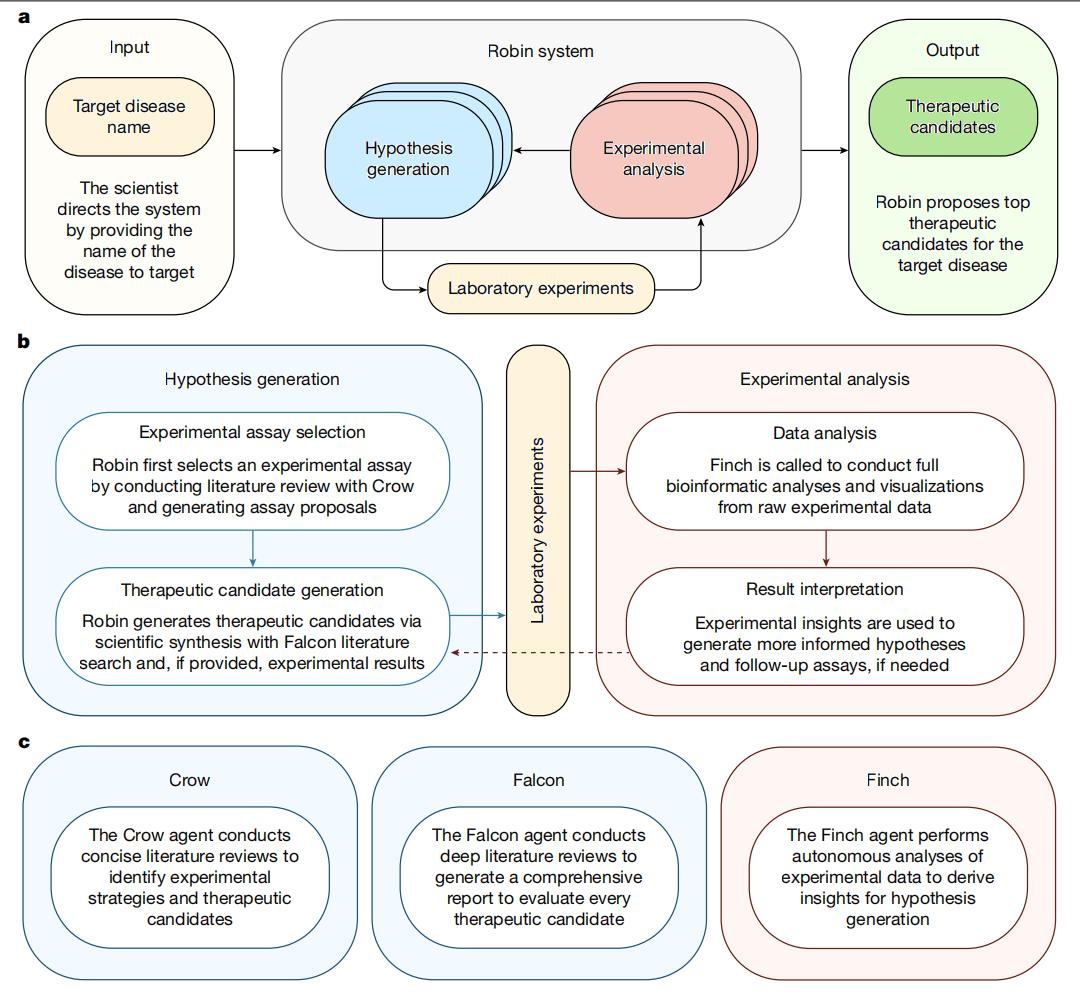
\includegraphics[width=\linewidth,height=4.8cm,keepaspectratio]{architecture_robin.png}
    \caption{Robin architecture}
    \end{figure}
\end{column}
\begin{column}{0.39\textwidth}
    \textbf{MAS}
    \begin{itemize}
        \setlength{\itemsep}{0.35em}
        \item Crow / Falcon:\\PaperQA2
        \item Finch:\\Jupyter kernel
    \end{itemize}
    \medskip
    \textbf{Evaluation}
    \begin{itemize}
        \setlength{\itemsep}{0.35em}
        \item Position bias in LLM judges
        \item Tournament
        \item Bradley--Terry--Luce (BTL)
    \end{itemize}
    \medskip
    \textbf{Prompt engineering}
\end{column}
\end{columns}
\end{frame}

